% ============================================================================
% Procedimiento de ensayo RE-TP-001
% Base: esquema del procedimiento de Emisiones Radiadas provisto por la catedra.
% Un solo archivo .tex. Necesita en la misma carpeta: logo_fiuba.png,
% logo_materia.png, fig_esquema_general.png, fig_camara_anecoica.png y
% fig_camara_semianecoica.png.
% Compilar con pdfLaTeX (Overleaf: Menu > Compiler > pdfLaTeX).
% ============================================================================
\documentclass[11pt,a4paper]{article}

\usepackage[utf8]{inputenc}
\usepackage[T1]{fontenc}
\usepackage[spanish,es-tabla,es-nodecimaldot]{babel}
\usepackage[a4paper,margin=2.5cm,headheight=14pt]{geometry}
\usepackage{graphicx}
\usepackage{float}       % permite la opcion [H] en figuras y tablas
\usepackage{booktabs}
\usepackage{array}
\usepackage{longtable}
\usepackage{enumitem}
\usepackage{amsmath}
\usepackage{xcolor}
\usepackage{fancyhdr}
\usepackage{tikz}
\usetikzlibrary{babel}   % evita el choque entre TikZ y los atajos < > del español
\usepackage[hidelinks]{hyperref}

% ---------------------------------------------------------------- datos ----
\newcommand{\codigo}{RE-TP-001}
\newcommand{\version}{1.1 (borrador)}
\newcommand{\fecha}{5 de octubre de 2026}

% Texto que hay que completar o confirmar antes de usar el documento
\newcommand{\pendiente}[1]{\textcolor{red}{[#1]}}
% Casillero vacio para completar a mano
\newcommand{\casilla}{\rule{0pt}{4.2ex}}

\pagestyle{fancy}
\fancyhf{}
\lhead{\small \codigo{} -- Procedimiento de ensayo de Emisiones Radiadas (RE)}
\rhead{\small Versión \version}
\cfoot{\small \thepage}

\setlist{itemsep=2pt,topsep=4pt}

\begin{document}

% ============================================================== caratula ====
\begin{titlepage}
  \centering
  \vspace*{0.5cm}
  % logo de la facultad a la izquierda y logo de la materia a la derecha
  \begin{minipage}[c]{0.56\textwidth}
    \centering
    
\includegraphics[width=\textwidth]{logo_fiuba.png}
  \end{minipage}\hfill
  \begin{minipage}[c]{0.34\textwidth}
    \centering
    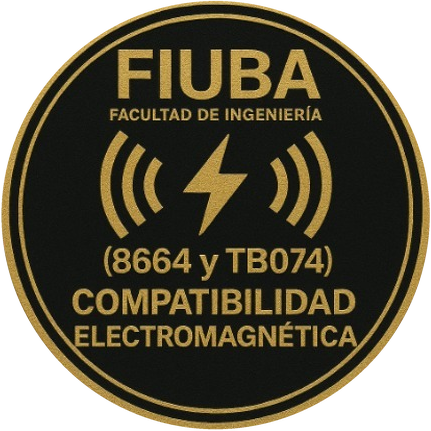
\includegraphics[width=\textwidth]{logo_materia.png}
  \end{minipage}\par
  \vspace{0.8cm}
  {\large Universidad de Buenos Aires -- Facultad de Ingeniería\par}
  {\large Compatibilidad Electromagnética (8664 y TB074)\par}
  \vspace{1.6cm}
  {\Large \textsc{Procedimiento de ensayos}\par}
  \vspace{0.3cm}
  {\LARGE \bfseries Emisiones Radiadas (RE)\par}
  \vspace{0.6cm}
  {\Large Comb Generator basado en Software Defined Radio (SDR)\par}
  \vspace{0.8cm}
  {\large Código: \textbf{\codigo} \qquad Versión: \textbf{\version}\par}
  \vfill
  \begin{tabular}{ll}
    \toprule
    Autor               & Martín Ledesma \\
    Docentes            & Pablo Marino Belcaguy \\
                        & Walter Gustavo Fano \\
    Laboratorio         & CETEM, Florencio Varela \\
    Asistencia          & Federico Martinez (CETEM) \\
    Fecha               & \fecha \\
    \bottomrule
  \end{tabular}
  \vspace{1cm}
\end{titlepage}

% ====================================================== control de cambios ==
\section*{Control de versiones}
\begin{tabular}{@{}llp{8cm}@{}}
  \toprule
  Versión & Fecha & Cambios \\
  \midrule
  1.0 (borrador) & \fecha & Primera emisión. \\
  \bottomrule
\end{tabular}

\section*{Participantes}
\begin{tabular}{@{}lp{10cm}@{}}
  \toprule
  Persona & Función en el ensayo \\
  \midrule
  Martín Ledesma        & Opera la SDR y el software y registra los resultados. \\
  Federico Martinez     & Opera la cámara, el mástil, la mesa y el receptor del CETEM. \\
  Pablo Marino Belcaguy & Docente, revisión del procedimiento. \\
  Walter Gustavo Fano   & Docente, revisión del procedimiento. \\
  \bottomrule
\end{tabular}

\tableofcontents
\newpage

% ============================================================================
\section*{Procedimiento de ensayos Emisiones Radiadas (RE)}

Para evaluar las emisiones radiadas de un Comb Generator basado en SDR bajo normativas estándar de compatibilidad electromagnética (CISPR 32 / ANSI C63.4), se estructura un Procedimiento de Ensayo de Emisiones Radiadas (\emph{Radiated Emissions Test Procedure}) estándar de laboratorio.

\begin{figure}[H]
  \centering
  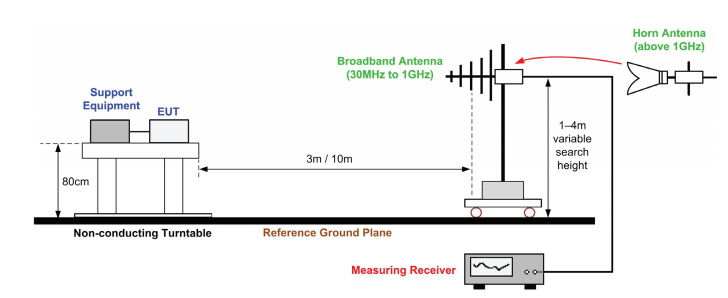
\includegraphics[width=0.85\textwidth]{fig_esquema_general.png}
  \caption{Disposición general de un ensayo de emisiones radiadas.}
\end{figure}

\begin{figure}[H]
  \centering
  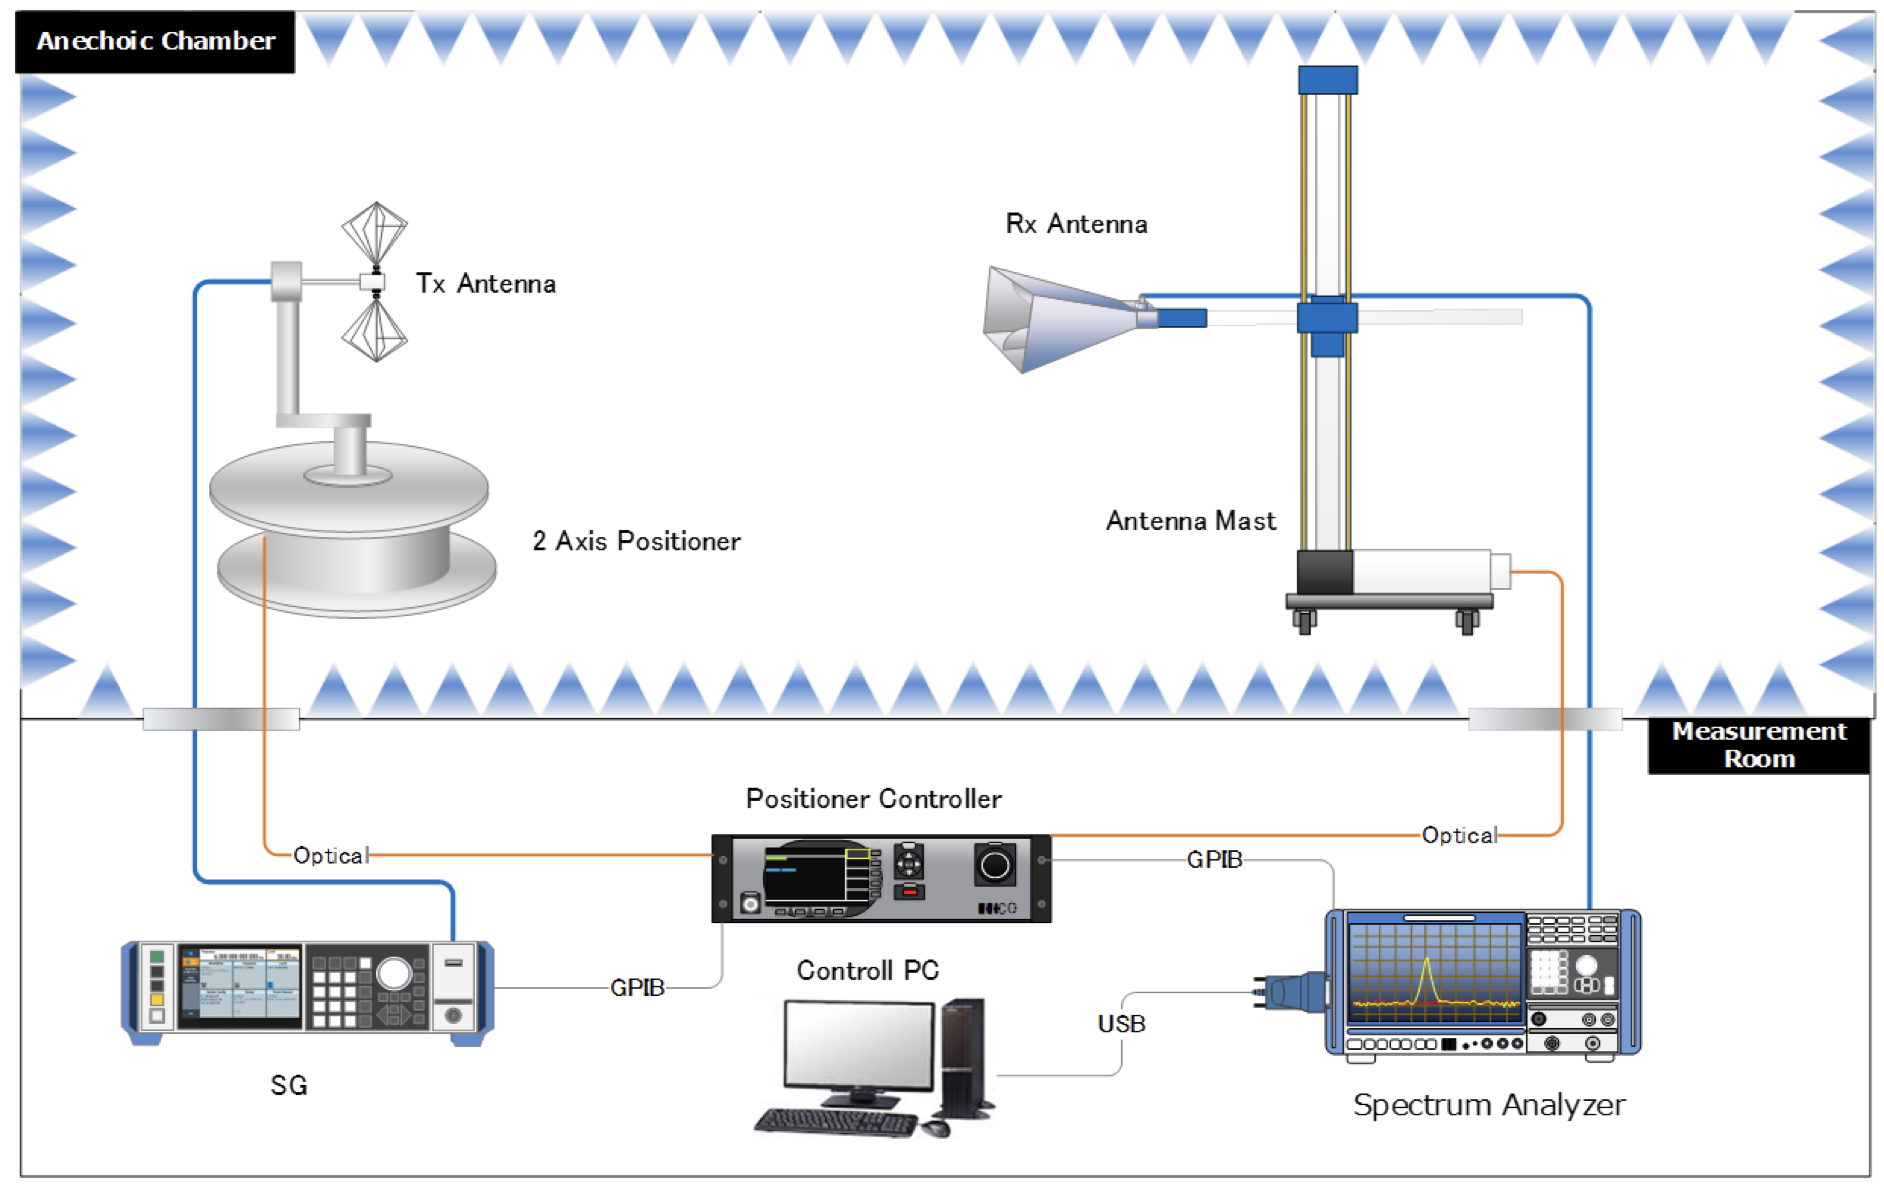
\includegraphics[width=0.85\textwidth]{fig_camara_anecoica.png}
  \caption{Cámara y sala de medición.}
\end{figure}

\newpage
\begin{center}
  {\large\bfseries PROCEDIMIENTO DE ENSAYO DE EMISIONES RADIADAS (\codigo)}
\end{center}

% ============================================================================
\section{Objeto y alcance}

Este documento define los pasos para la caracterización y verificación de emisiones radiadas en el dominio de la frecuencia del equipo \textbf{EUT/DUT: Comb Generator basado en Software Defined Radio (SDR)}.

\begin{itemize}
  \item \textbf{Normas de referencia aplicables:} CISPR 16-2-3, CISPR 32 (Clase B / Clase A), ANSI C63.4.
  \item \textbf{Rango de frecuencia:} 60~MHz a 980~MHz en esta primera versión (ampliable según la frecuencia máxima transmitida por el SDR).
\end{itemize}

\paragraph{Finalidad.} El Comb Generator se usa como \emph{fuente de referencia} para verificar la cadena de medición de emisiones radiadas del laboratorio y controlar su continuidad en el tiempo. Emite 24 líneas entre 60 y 980~MHz, una cada 40~MHz, calibradas por conducción a 0~dBm~$\pm$~1~dB. La primera medición en la cámara establece la \emph{curva de referencia}, mientras que las mediciones posteriores se comparan contra ella. Si el mismo peine, montado de la misma forma, se recibe distinto, lo que cambió es la cadena de medición.

\begin{itemize}
  \item \textbf{Qué verifica:} la cadena completa: cámara, antena de medición, cables y receptor.
  \item \textbf{Límites normativos:} el peine es un emisor intencional, por lo que el resultado no se evalúa como conformidad con CISPR~32. El límite puede dibujarse en el gráfico como línea de referencia.
  \item \textbf{Validez:} los resultados valen para el montaje descrito en la sección~\ref{sec:montaje}. Cambiar la antena transmisora, su posición o el recorrido del cable USB obliga a tomar una curva de referencia nueva.
\end{itemize}

% ============================================================================
\section{Equipamiento y medios de ensayo}

\begin{itemize}
  \item \textbf{Entorno:} Cámara Semianecoica calibrada a 3 metros.
  \item \textbf{Receptor EMI:} Cumplimiento con CISPR 16-1-1.
  \item \textbf{Modo:} Detector Quasi-Peak y Peak, RBW 120~kHz de 30~MHz a 1~GHz; RBW 1~MHz por encima de 1~GHz. En este procedimiento se usa el detector Peak con MAX HOLD (ver sección~\ref{sec:pasos}).
  \item \textbf{Antenas de Medición:}
        \begin{itemize}
          \item Biconical (30~MHz -- 300~MHz).
          \item Log-Periodic / Bilog Hybrid (30~MHz -- 1~GHz).
          \item Horn.
          \item Mástil de antena motorizado (1~m a 4~m de altura).
        \end{itemize}
  \item \textbf{Mesa Giratoria (Turntable):} a 0,8~m de altura respecto al plano de masa.
  \item \textbf{Cables:} USB 3.0 de alta velocidad y larga distancia.
  \item \textbf{SDR} con sus accesorios para poder utilizarla, incluyendo la antena, e incluyendo shield que evite interferencias de la misma SDR.
        \begin{itemize}
          \item bladeRF 2.0 micro xA9, número de serie \texttt{321e0fa5875945d99b11070bb0a76d31}.
          \item Antena transmisora: telescópica de 30~cm, totalmente extendida (hasta el tope) y vertical, en el conector TX1. Siempre la misma y siempre extendida igual.
          \item Caja metálica: \pendiente{falta definir}.
          \item Ferrita para el cable USB.
        \end{itemize}
  \item \textbf{Software asociado a la SDR:} GNU Radio 3.10, con:
        \begin{itemize}
          \item el flujo \texttt{exp25\_a9\_peine\_con\_silencio\_desde60.grc};
          \item el archivo de calibración \texttt{calibracion\_peine\_desde60.txt}.
        \end{itemize}
  \item \textbf{Computadora} para manejar la SDR desde afuera, conectada por el cable USB instalado entre la sala de control y la cámara.
  \item Analizador de espectro portátil (tinySA Ultra) y cable coaxial, para verificar la fuente por conducción antes de entrar a la cámara.
\end{itemize}

\paragraph{Referencias.}
\begin{itemize}
  \item YRS03, Eurofins York, Comb Generator: referencia comercial del tipo de fuente.
  \item bladeRF 2.0 micro, Nuand. Potencia de salida CW: +8~dBm.
\end{itemize}

\paragraph{Precauciones.}
\begin{itemize}
  \item Emitir solo dentro de la cámara: el peine cae sobre bandas de radiodifusión, aeronáutica y telefonía. Fuera de la cámara la SDR se conecta únicamente por cable a un analizador.
  \item Analizador portátil: atenuación interna fija en 30~dB antes de subir la ganancia de la SDR a 55 o 65~dB.
  \item Nunca conectar la salida TX de la SDR a su entrada RX.
  \item El software arranca en \textsc{pausa}. Destildarla solo con el montaje terminado y la cámara cerrada.
  \item Si el programa se cierra solo o muestra errores de USB, desenchufar la SDR, esperar un minuto y volver a enchufarla.
\end{itemize}

% ============================================================================
\section{Configuración del DUT}\label{sec:montaje}

\begin{figure}[H]
  \centering
  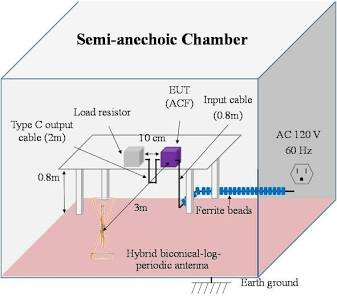
\includegraphics[width=0.55\textwidth]{fig_camara_semianecoica.png}
  \caption{Montaje de un equipo de mesa en la cámara semianecoica.}
\end{figure}

Colocar el SDR (Comb Generator) sobre la mesa giratoria no conductiva a $0{,}8$~m sobre el plano de tierra reflejante.

Cables de alimentación / control: si el SDR requiere conexión USB/Power a una PC host, la PC debe ubicarse fuera de la cámara o blindarse debidamente. Si se usan cables dentro de la cámara, colocar un filtro/ferrita según marca la norma ANSI C63.4 para evitar que los cables actúen como antenas no deseadas.

Configurar el script del SDR para emitir el patrón de peine deseado. En este procedimiento el patrón es el descrito en la sección~\ref{sec:sdr}: 24 líneas de 60 a 980~MHz, una por vez.

\paragraph{Geometría fija.} La medición de rutina se hace sin girar la mesa ni barrer la altura: así el resultado no depende de encontrar un máximo y es más repetible. La geometría se elige una sola vez, en el barrido preliminar (paso~\ref{paso:prescan}).

\begin{figure}[H]
  \centering
  \begin{tikzpicture}[font=\small,>=latex]
    \draw[line width=1.2pt] (-1,0) -- (11,0);
    \node[below] at (5,0) {Plano de tierra reflectante};
    \draw (0.2,0) -- (0.2,1.6) (1.8,0) -- (1.8,1.6);
    \draw[line width=1pt] (0,1.6) -- (2,1.6);
    \draw[fill=gray!25] (0.7,1.6) rectangle (1.3,1.9);
    \draw[line width=0.8pt] (1.0,1.9) -- (1.0,2.6);
    \node[above] at (1.0,2.6) {SDR + antena};
    \draw[<->] (-0.4,0) -- (-0.4,1.6) node[midway,left] {0,8 m};
    \draw[dashed] (0.7,1.7) -- (0.45,1.7) -- (0.45,0.05) -- (-1,0.05);
    \node[left] at (-1,0.05) {USB a la PC};
    \draw[line width=1pt] (9,0) -- (9,3.4);
    \draw[line width=0.8pt] (8.2,3.0) -- (9,3.0);
    \foreach \x/\h in {8.25/0.45,8.45/0.38,8.65/0.30,8.85/0.22}
      \draw (\x,3.0-\h) -- (\x,3.0+\h);
    \node[above] at (8.9,3.5) {Antena de medición};
    \draw[<->] (9.5,0) -- (9.5,3.0) node[midway,right] {altura fija};
    \draw[<->] (1.0,0.6) -- (9,0.6) node[midway,above] {3 m};
    \draw (9,0.05) -- (11,0.05);
    \node[right] at (11,0.05) {al receptor};
  \end{tikzpicture}
  \caption{Montaje usado en este procedimiento. La PC y el receptor quedan fuera de la cámara.}
\end{figure}

\begin{enumerate}
  \item Colocar la SDR en el centro de la mesa, con la antena transmisora vertical.
  \item Bajar el cable USB recto hasta el piso y llevarlo al pasamuros siempre por el mismo recorrido. Colocar la ferrita junto a la SDR.
  \item Ubicar la antena de medición a 3~m, a la altura fija elegida.
  \item Fotografiar el montaje desde dos lados. Las fotos forman parte de la curva de referencia: en cada medición posterior el montaje se arma igual que en las fotos.
\end{enumerate}

\begin{table}[H]
  \centering
  \begin{tabular}{@{}lll@{}}
    \toprule
    Parámetro & Valor por defecto & Valor usado \\
    \midrule
    Distancia de medición           & 3~m      & \pendiente{completar} \\
    Altura de la mesa               & 0,8~m    & \pendiente{completar} \\
    Ángulo de la mesa               & 0\textdegree & \pendiente{completar} \\
    Altura de la antena de medición & 1,5~m    & \pendiente{completar} \\
    Polarizaciones                  & H y V    & \pendiente{completar} \\
    Orientación de la SDR           & conector TX hacia la antena & \pendiente{completar} \\
    \bottomrule
  \end{tabular}
  \caption{Geometría fija. Los valores usados se definen en la primera medición.}
  \label{tab:geometria}
\end{table}

% ============================================================================
\section{Procedimiento paso a paso}\label{sec:pasos}

Los ajustes del receptor son los de la sección~\ref{sec:protocolo}, paso~2. Antes de entrar a la cámara se verifica la fuente por conducción (anexo~\ref{anexo:previa}).

\begin{enumerate}[label=\textbf{\arabic*.},leftmargin=*,itemsep=8pt]

  \item \textbf{Medición del Ruido de Fondo (Ambient Noise):} Verificación previa del entorno.

        Desactivar o apagar el SDR.

        Ejecutar un barrido rápido en detector Peak desde 30~MHz hasta la máxima frecuencia de interés. Verificar que el nivel de ruido ambiental esté al menos \textbf{6~dB por debajo} de los límites normativos aplicables. Se verifica entonces que el ruido quede al menos 10~dB por debajo del nivel con que después se reciben las líneas del peine. Guardar la traza.

  \item\label{paso:prescan} \textbf{Barrido Preliminar (Prescan):} Identificación de armónicos del Comb Generator.
        \begin{enumerate}[label=\arabic*.]
          \item Encender la SDR sin modo COMB, en modo stand by, y se mide todo. En el software: ejecutar el flujo y dejarlo en \textsc{pausa}. Tomar una traza en MAX HOLD durante un minuto y guardarla: muestra lo que emite la placa por sí sola (su reloj y el USB).
          \item Poner la SDR en modo de generación de ``Comb'': calibración importada, ganancia 65~dB, destildar \textsc{pausa}.
          \item Configurar el receptor EMI en \textbf{Max Hold (Peak)} con un barrido rápido.
          \item Girar la mesa 360\textdegree{} continuamente y variar la altura de la antena entre 1~m y 4~m en ambas polarizaciones (Horizontal y Vertical) para mapear los picos principales del peine de frecuencias.
        \end{enumerate}
        El punto 4 se hace \textbf{solo la primera vez}. Su resultado es la geometría fija: una altura y un ángulo donde las 24 líneas se reciben bien y ninguna cae en un mínimo. Anotarlos en la tabla~\ref{tab:geometria}. Si no hay tiempo, usar los valores por defecto.

  \item \textbf{Medición Final:} con la geometría fija.
        \begin{enumerate}[label=\arabic*.]
          \item Mesa y antena de medición en la posición de la tabla~\ref{tab:geometria}, polarización horizontal.
          \item Reiniciar MAX HOLD. Anotar el número de paso que muestra la ventana del software y esperar a que vuelva a ese mismo número: es una pasada completa (4~min~48~s).
          \item Guardar la traza (imagen y datos).
          \item Repetir con polarización vertical.
          \item Leer el nivel de las 24 líneas en cada polarización y completar la tabla de la sección~\ref{sec:registro}.
        \end{enumerate}

        \emph{Maximización (cumplimiento con CISPR / ANSI).} El método normativo, para cada armónico o frecuencia crítica identificada en el Prescan, es:
        \begin{enumerate}[label=\arabic*.]
          \item Posicionar la mesa en el ángulo $\theta$ donde la emisión sea máxima.
          \item Elevar/bajar el mástil de antena entre 1~m y 4~m para encontrar el pico por interferencia con el suelo.
          \item Cambiar la polarización de la antena (Horiz / Vert) para encontrar el nivel máximo de $E_{radiado}$.
          \item Aplicar el detector \textbf{Quasi-Peak (QP)} con tiempo de integración de 1~segundo por punto.
        \end{enumerate}
        En esta versión no se aplica en la medición de rutina, por dos motivos: para controlar continuidad interesa repetir siempre la misma geometría, y el generador emite una línea por vez (6~s cada 12~s), lo que no permite detenerse en una línea para maximizarla ni medirla en cuasi-pico. Queda como ampliación.

  \item \textbf{Repetibilidad (solo la primera vez).} Desmontar todo, volver a montar siguiendo las fotos y repetir la medición final. La diferencia entre las dos es la repetibilidad del montaje, y sirve para confirmar o ajustar las tolerancias de la sección~\ref{sec:criterio}.

  \item \textbf{Cálculo de Campo Eléctrico Real:} El valor final de campo eléctrico medido $E_{dB\mu V/m}$ se calcula como:
        \begin{equation}
          E_{dB\mu V/m} = V_{receptor}\,(dB\mu V) + AF\,(dB/m)
            + L_{cable}\,(dB) - G_{amp}\,(dB)
        \end{equation}

        Para controlar continuidad alcanza con comparar la lectura del receptor, siempre que $AF$, $L_{cable}$ y $G_{amp}$ sean los mismos que en la curva de referencia. Un cambio en cualquiera de ellos es justamente lo que este procedimiento detecta; por eso se anotan en el registro.
\end{enumerate}

\paragraph{Cierre.} Tildar \textsc{pausa}, cerrar el programa y desenchufar la SDR. Guardar capturas, fotos y el registro en una carpeta con la fecha.

% ============================================================================
\section{Registro y reporte}\label{sec:registro}

\begin{itemize}
  \item Gráfica del espectro completo ($30~MHz - 1~GHz$) comparado contra el límite de la norma elegida (CISPR 32 Class B). El límite se dibuja solo como referencia; junto a él se grafica la curva de referencia del peine.
  \item Tabla de picos con: Frecuencia, Nivel medido, Referencia, Diferencia ($dB$), Ángulo de mesa (\textdegree), Altura de antena ($m$) y Polarización ($H/V$). Con geometría fija, ángulo y altura son los mismos para todas las líneas y se anotan una sola vez.
  \item Trazas del ruido de fondo y de la emisión propia de la SDR, fotos del montaje y captura de la verificación previa por conducción.
\end{itemize}

\subsection{Criterio de aceptación}\label{sec:criterio}

Para cada línea y cada polarización se calcula la diferencia entre el nivel medido y el de la curva de referencia.

\begin{table}[H]
  \centering
  \begin{tabular}{@{}ll@{}}
    \toprule
    Diferencia con la referencia & Resultado \\
    \midrule
    Hasta $\pm$3~dB          & Conforme \\
    Entre $\pm$3 y $\pm$6~dB & Revisar el montaje contra las fotos y repetir \\
    Más de $\pm$6~dB         & No conforme: investigar la cadena de medición \\
    \bottomrule
  \end{tabular}
  \caption{Criterio de continuidad. Valores iniciales, a confirmar con el paso de repetibilidad.}
\end{table}

Los 3~dB resultan de sumar la tolerancia de la fuente ($\pm$1~dB) y la repetibilidad esperada al volver a montar. Las líneas que no superen por 10~dB al ruido de fondo y a la emisión propia de la SDR se marcan y no se usan para el criterio.

Si varias líneas contiguas se apartan en el mismo sentido, conviene sospechar de un elemento con respuesta en frecuencia (antena, cable, preamplificador). Si todas se apartan por igual, de una ganancia o una atenuación. Si la verificación previa por conducción no dio 0~dBm~$\pm$~1~dB, el problema está en la fuente y no en la cadena.

\subsection{Planilla}

\begin{tabular}{@{}p{6.3cm}p{8.5cm}@{}}
  \toprule
  Fecha y hora                         & \casilla \\
  Operadores                           & \casilla \\
  ¿Curva de referencia o verificación? & \casilla \\
  Receptor, antena y cables usados     & \casilla \\
  Preamplificador (sí/no, ganancia)    & \casilla \\
  Ángulo de mesa y altura de antena    & \casilla \\
  Fecha de la calibración de la fuente & \casilla \\
  Verificación previa: rango de las 24 líneas por conducción (dBm) & \casilla \\
  Tiempo de barrido del receptor       & \casilla \\
  Archivos guardados                   & \casilla \\
  \bottomrule
\end{tabular}

\vspace{0.5cm}

\begin{longtable}{@{}c|cc|cc|cc|c@{}}
  \toprule
  Frecuencia & \multicolumn{2}{c|}{Nivel medido} & \multicolumn{2}{c|}{Referencia} & \multicolumn{2}{c|}{Diferencia (dB)} & Resultado \\
  (MHz) & H & V & H & V & H & V & \\
  \midrule
  \endhead
  \bottomrule
  \endfoot
   60 & & & & & & & \\
  100 & & & & & & & \\
  140 & & & & & & & \\
  180 & & & & & & & \\
  220 & & & & & & & \\
  260 & & & & & & & \\
  300 & & & & & & & \\
  340 & & & & & & & \\
  380 & & & & & & & \\
  420 & & & & & & & \\
  460 & & & & & & & \\
  500 & & & & & & & \\
  540 & & & & & & & \\
  580 & & & & & & & \\
  620 & & & & & & & \\
  660 & & & & & & & \\
  700 & & & & & & & \\
  740 & & & & & & & \\
  780 & & & & & & & \\
  820 & & & & & & & \\
  860 & & & & & & & \\
  900 & & & & & & & \\
  940 & & & & & & & \\
  980 & & & & & & & \\
\end{longtable}

\noindent Observaciones: \\[1.6cm]

% ============================================================================
\section{Espaciado recomendado por banda normativa}

Para no perder picos de emisión ni solapar armónicos dentro de la ventana de medición, el SDR debe programarse con los siguientes espaciados recomendados:

\begin{table}[H]
  \centering
  \begin{tabular}{@{}p{2.7cm}p{2.0cm}p{2.9cm}p{6.4cm}@{}}
    \toprule
    Banda de frecuencia & RBW normativo (CISPR) & Espaciado recomendado ($f_0$) & Justificación EMC \\
    \midrule
    30~MHz a 300~MHz & 120~kHz & 1~MHz a 5~MHz & Permite evaluar con alta densidad la zona crítica de resonancia de cables y antenas Biconical. \\
    300~MHz a 1~GHz  & 120~kHz & 10~MHz a 20~MHz & Garantiza suficientes líneas de prueba sin saturar la pantalla ni sobrecargar la velocidad del barrido. \\
    $>$ 1~GHz (si aplica) & 1~MHz & 50~MHz a 100~MHz & Adecuado para la banda microondas con filtros Log-Periodic o Horn. \\
    \bottomrule
  \end{tabular}
  \caption{Espaciado recomendado del peine según la banda.}
\end{table}

\textbf{Regla de oro metrológica:} El espaciado del peine ($f_0$) debe ser \textbf{al menos 5 a 10 veces mayor que el RBW del receptor} ($f_0 \gg RBW$) para que el detector del receptor mida cada armónico de forma individual y no sume potencia de líneas adyacentes.

\paragraph{Espaciado adoptado en esta versión: 40~MHz en toda la banda.}

Cumple la regla de oro con margen (más de 300 veces el RBW de 120~kHz), pero es más ancho que el recomendado en la tabla, sobre todo por debajo de 300~MHz. Se adoptó por una limitación de la SDR, que es que su mezclador repite cada línea alrededor de los armónicos impares de la portadora, entre 9 y 28~dB por debajo. Con líneas cada 40~MHz desde 60~MHz y la portadora 10~MHz por encima de la línea, esas repeticiones caen exactamente sobre otras líneas del peine y MAX HOLD las tapa. Este espaciado es el valor óptimo dentro del cual no hay perdidas de paquetes entre la PC y la SDR ($<40MSPS$). Densificar la banda baja queda como mejora.

% ============================================================================
\section{Cálculo y configuración en el SDR}\label{sec:sdr}

La SDR no puede generar pulsos de 1~ns: su tasa de muestreo máxima es 61,44~MSPS y en la PC usada el enlace USB sostiene 40~MSPS, o sea unos 36~MHz de ancho de banda instantáneo. Por eso el peine se arma \emph{por saltos}, trasladando la señal con el oscilador local. La SDR emite una línea por vez y el receptor, en MAX HOLD, las acumula hasta mostrar el peine completo.

\begin{table}[H]
  \centering
  \begin{tabular}{@{}lp{8.6cm}@{}}
    \toprule
    Parámetro & Valor \\
    \midrule
    Líneas                        & 24: 60, 100, 140, \dots, 980~MHz \\
    Separación entre líneas ($f_0$) & 40~MHz \\
    Portadora de cada línea       & línea + 10~MHz (70, 110, \dots, 990~MHz) \\
    Tasa de muestreo              & 40~MSPS, filtro de 36~MHz \\
    Tiempo por línea              & 6~s encendida + 6~s apagada \\
    Salto de frecuencia           & en la mitad del silencio \\
    Pasada completa               & 4~min~48~s \\
    Nivel de calibración (conducido)   & 0~dBm por línea, con ganancia de TX 65~dB \\
    Nivel de transmisión (irradiado)   & 3~dBm por línea, con ganancia de TX 65~dB \\
    Planitud medida (conducido)   & 1,1~dB entre la línea más alta y la más baja \\
    \bottomrule
  \end{tabular}
  \caption{Parámetros del generador peine (flujo de GNU Radio del EXP-25).}
\end{table}

\paragraph{Condición para el receptor.} Cada línea está encendida 6~s. Para que al menos un barrido completo caiga dentro de ese tiempo, el barrido del receptor debe durar \textbf{menos de 3~s}. Si dura más, hay que aumentar el tiempo por línea en el software (variable \texttt{permanencia}) a más del doble del tiempo de barrido.

% ============================================================================
\section{Protocolo de verificación paso a paso en el laboratorio}\label{sec:protocolo}

\begin{enumerate}[label=\textbf{Paso \arabic*:},leftmargin=*,itemsep=8pt]

  \item \textbf{Generación del Peine Normativo en SDR:} Configuración de parámetros en el software del SDR.
        \begin{enumerate}[label=\arabic*.]
          \item Ajustar el \emph{Sample Rate} del DAC del SDR al valor máximo que el enlace sostiene sin pérdida de muestras: 40~MSPS en este montaje (el LED de la placa debe quedar encendido fijo).
          \item Cargar la secuencia del peine: en esta versión no es un tren de pulsos sino un tono por portadora, con las amplitudes de la calibración (botón \emph{Importar calibración previa}).
        \end{enumerate}

  \item \textbf{Configuración del Receptor según CISPR 16:} Ajustes en el Analizador de Espectro / Receptor EMI.
        \begin{enumerate}[label=\arabic*.]
          \item Ajustar la frecuencia de inicio a $30~MHz$ y parada a $1~GHz$.
          \item Configurar el \textbf{RBW en 120~kHz} y \textbf{VBW en 300~kHz}.
          \item Seleccionar el detector en \textbf{Max Hold (Peak)}.
          \item Verificar que el tiempo de barrido sea menor a 3~s.
        \end{enumerate}

  \item \textbf{Verificación de Picos y Resolución:}
        \begin{enumerate}[label=\arabic*.]
          \item Comprobar que en la pantalla se observen picos equidistantes exactamente cada $40~MHz$ ($60, 100, 140, \dots, 980$~MHz).
          \item Verificar que la relación Señal/Ruido ($SNR$) de cada armónico sea de al menos 10~dB a 15~dB por encima de las fugas de portadoras y del piso de ruido.
        \end{enumerate}
\end{enumerate}

% ============================================================================
\appendix

\section{Verificación previa de la fuente, por conducción}\label{anexo:previa}

Se hace fuera de la cámara, antes de cada medición. Separa un cambio en la fuente de un cambio en la cadena.

\begin{enumerate}
  \item Conectar la salida TX1 de la SDR al analizador portátil con el cable coaxial. Analizador: 45 a 1005~MHz, RBW 300~kHz, atenuación 30~dB, MAX HOLD.
  \item Abrir el flujo, ejecutarlo, apretar \emph{Importar calibración previa}, elegir ganancia 65~dB y destildar \textsc{pausa}.
  \item Reiniciar MAX HOLD y esperar una pasada completa (4~min~48~s).
  \item \textbf{Criterio:} las 24 líneas deben estar en 0~dBm~$\pm$~1~dB. Si alguna no lo está, corregir su contador o generar la calibración de nuevo (anexo~\ref{anexo:cal}) antes de seguir.
  \item Tildar \textsc{pausa} y guardar la captura.
\end{enumerate}

\section{Manejo del software}\label{anexo:sw}

La ventana del flujo muestra en todo momento la etapa, la línea que está saliendo, su portadora y el número de paso dentro de la pasada.

\begin{description}
  \item[PAUSA] Con la casilla tildada la salida queda en silencio. El programa arranca así.
  \item[Ganancia de TX] 45, 55 o 65~dB: líneas calibradas en $-20$, $-10$ o 0~dBm. La calibración vale para las tres.
  \item[Nivel] \emph{Calibrado} o \emph{Calibrado + 3~dB}. La segunda opción sube todas las líneas; en la medición por conducción dieron +2,3~dBm de media, porque la placa ya comprime un poco.
  \item[Importar calibración previa] Carga en los 24 contadores los valores del archivo de calibración.
  \item[Guardar calibración] Escribe en el archivo los valores que están en los contadores.
  \item[Generar calibración] Arma la calibración a partir de una captura del analizador (anexo~\ref{anexo:cal}).
  \item[Contadores] Uno por línea. Guardan el nivel leído con el peine sin calibrar, menos 20~dB. Para bajar una línea $x$~dB se le suma $x$ a su contador; para subirla, se le resta.
\end{description}

El 3er LED (de izquierda a derecha) de la SDR debe quedar encendido fijo mientras el flujo corre. Si titila, a la placa le están faltando muestras por el USB y la medición no es válida.

\section{Calibración de la fuente por conducción}\label{anexo:cal}

Se hace con la SDR conectada por cable al analizador portátil (atenuación 30~dB, 45 a 1005~MHz, RBW 300~kHz, MAX HOLD).

\begin{enumerate}
  \item Abrir el flujo y ejecutarlo \emph{sin importar ninguna calibración}: los 24 contadores deben estar en cero.
  \item Elegir ganancia 65~dB y destildar \textsc{pausa}.
  \item Reiniciar MAX HOLD, esperar una pasada completa y guardar la captura en formato \texttt{.csv}.
  \item Reiniciar MAX HOLD y guardar una segunda captura de otra pasada. Con dos capturas el programa descarta los picos momentáneos.
  \item Apretar \emph{Generar calibración} y elegir las dos capturas a la vez. El programa busca el pico de cada línea, carga los contadores y guarda el archivo de calibración.
  \item Reiniciar MAX HOLD, esperar una pasada y verificar que las 24 líneas queden en 0~dBm~$\pm$~1~dB. Si alguna no lo cumple, corregir su contador a mano y apretar \emph{Guardar calibración}.
\end{enumerate}

La calibración vale para el cable y el analizador con que se hizo. Lleva unos 20~minutos.

\end{document}
